% !TEX root=../../mt-motion-analysis.tex
%!TeX spellcheck = en-US
\chapter{Methods}
\section{Overview}
In this chapter the system for assessing POEs will be presented. This system is naturally divided into two parts where firstly the videos are analyzed. The first subsystem extracts body part coordinates of the subjects. This information is then passed to the second subsystem where it is used to calculate a score according to \cite{Nae2017}. The data is presented in Section \ref{sec:met-data} and the two subsystems are described in Sections \ref{sec:met-loc} and \ref{sec:met-class} respectively.

\section{Data}\label{sec:met-data}
The data available is in the form of videos each containing one subject, recorded from the front, performing three-five repetitions of specific motions. The motions are \textit{Single-leg squat, Forward lunge, Stair descending, Forward lunge, Single leg hop for distance, and Side hop}. Each motion has a number of POE scores associated with them. The motion-POE combinations are shown in Table \ref{tab:met:motion-poes}. In Sections \ref{sec:met-SLS}-\ref{} the motions and POEs evaluated in this project are described.

% The videos were recorded with different orientations and frame rates.
%
% The available videos has been assessed by a physiotherapist and for each repetition in each motion a number of POE scores has been awarded.


\begin{table}
 \centering
 \caption{Motion-POE combinations available in the data.}
 \label{tab:met:motion-poes}

 \begin{tabular}{|c|ccccc|}
  \hline
  \backslashbox{POE}{Motion}                      &
  \multicolumn{1}{c}{\begin{tabular}[c]{@{}c@{}}Single\\ leg squat\end{tabular}}   &
  \multicolumn{1}{c}{\begin{tabular}[c]{@{}c@{}}Stair\\ descending\end{tabular}}   &
  \multicolumn{1}{c}{\begin{tabular}[c]{@{}c@{}}Forward\\ lunge\end{tabular}}   &
  \multicolumn{1}{c}{\begin{tabular}[c]{@{}c@{}}Single leg hop\\ for distance\end{tabular}}   &
  \multicolumn{1}{c|}{\begin{tabular}[c]{@{}c@{}}Side\\ hop\end{tabular}}                      \\ \hline \hline

  Trunk                                           & x & x &   & x & x \\ \hdashline
  Hip                                             & x & x & x & x & x \\ \hdashline
  \multicolumn{1}{|c|}{\begin{tabular}[c]{@{}c@{}}Femoral\\ valgus\end{tabular}} &
  x                                               & x & x & x & x     \\ \hdashline
  \multicolumn{1}{|c|}{\begin{tabular}[c]{@{}c@{}}Knee medial to\\ foot position\end{tabular}} &
  x                                               & x & x & x & x     \\ \hdashline
  \multicolumn{1}{|c|}{\begin{tabular}[c]{@{}c@{}}Femur medial\\ to shank\end{tabular}} &
  x                                               & x & x & x & x     \\ \hdashline
  Foot                                            & x &   &   &   &   \\ \hline
 \end{tabular}
\end{table}

bara skriva om sls? om det bara 'r sls jag bed;mt.. ocks[ skriva det som avgr'nsningar

\subsection{Single-leg squat, SLS} \label{sec:met-SLS}
The subject performed a squat standing on one leg to a knee angle of approximately $60\degree$. The exercise was repeated five times and the entire movement was used to assess the POEs \cite{Nae2020}. An illustration is shown in Figure \ref{}.

\subsection{Stair descending, SD}
The subject stepped down from a 30 cm step board. The exercise was repeated five times and POEs were evaluated for the loaded leg during loading phase \cite{Nae2020}. An illustration is shown in Figure \ref{}.

\subsection{Forward Lunge, FL}

Helo I am now mispealing.



% The data the system is designed for is in the form of videos each containing around five repetitions of some specific motion. For each repetition in each motion up to five POEs has been graded according to \cite{Nae2017}.


\section{Body part localization} \label{sec:met-loc}
% \subsection{Preprocessing}
% ...
% rotation, flip etc
% \subsection{Pose estimation}
%The pose estimation can be seen as a feature extraction and dimensionality reduction.
The pose estimation is built around the open-source toolbox MMPose \cite{mmpose} from MMLab. Each frame is considered to be an independent image and is analyzed with the \gls{dark}-\gls{hrnet} trained on the \gls{coco}-wholebody dataset described in Section \ref{sec:pose_estimation}. % \ref{sec:hrnet, sec:dark, sec:coco}.

To get comparable results some of the videos were rotated and flipped before inferring the keypoints. This was needed since the videos were recorded in different orientations and the actions were performed with different legs. The rotations were based on the orientation of the subject (position of head w.r.t. the feet) in the first frame to have it standing up in the $y$-direction. Videos where the squats were performed with the left leg were then flipped around the $y$-axis to be able to use the same model for the left and right leg in a more efficient manner.

A bounding box for the subject is found using a Faster R-CNN model trained on the \gls{coco} dataset. This bounding box, including some margins around it, is resized to match the input size of the \gls{hpe} model used, which in our case was 384$\times$288 pixels. The final result of this is sequences with $x$- and $y$-coordinates of 17 keypoints per video frame.

%The file names contained information about which. The rotations were performed based on the position of the head with respect to the feet in the first frame.
\section{Classification} \label{sec:met-class}

\subsection{Preprocessing and dataset blabla..} \label{esc:met-class-preproc}
Before assessing the POEs based on the body part positions a number of preprocessing steps are conducted. Firstly the data is resampled as the videos are recorded with a number of different frame rates (25, 30, and 60Hz). The resampling is performed using linear interpolation to a new sample frequency of 25Hz. This data is then low pass filtered through a fourth order Butterworth filter with a cutoff frequency of 2.5Hz. PLOT P[ ;VERF;RING F;R FILTER? ELLER P[ FILTRERAD DATA?

While the POE assessment, see Section \ref{sec:met-class-...}, is performed on a per repetition basis the body part coordinates are extracted on a per video basis. Hence, each repetition should be extracted. This is done by finding peaks in the time series corresponding to certain body part positions. Which body part is used for this sequence splitting depends on which movement is analyzed. For SLS the $y$-coordinate of the right shoulder is used. The duration of each repetition varies significantly. With the duration of each repetition varying substantially between subjects padding in the time dimension is desirable. The reason for this is twofold, i) to simplify the handling of the data by storing it as a multidimensional array, and ii) to be able to train the eventual model in a more efficient manner using batches \cite{Goodfellow2016}. The padding is done by adding constant values of -1000 at the end of the sequences to some specified length. Details on how this is handled by the model are presented in Section \ref{sec:met-class-model}

BESKRIV ALGORITM F;R ATT DELA UPP I REPS

Finally the data is normalized to put the mean of the first five right hip-samples in the origin and the distance to the first five right shoulder-samples to one, according to \eqref{eq:met-normalization}.

\begin{align}
  \begin{split}
    (x,y)_i &= (x,y)_i - {\mean{(x,y)}}_{rh} \\
    (x,y)_i &= \frac{(x,y)_i}{\lVert \mean{(x,y)}_{rs} \rVert_2} \qquad , \forall i
  \end{split}
  \label{eq:met-normalization}
\end{align}
\begin{conditions}
    $\mean{(x,y)}_i$  & =   & mean over first five samples for body part $i$ \\
    \textit{rh}     & =   & right hip \\
    \textit{rs}     & =   & right shoulder \\
    \textit{i}      & \in & Available body parts %\{body parts\}
\end{conditions}

After these preprocessing steps a dataset $\in \mathbb{R}^{N \times T \times F}$ is created consisting of $N$ multivariate time series with $F$ channels of length $T$. The input channels can be $x$- and $y$-coordinates of body parts as well as angles between body parts.

\subsection{Models}
x-inception, coral osv. custom losses osv?

\begin{figure}
  \centering
  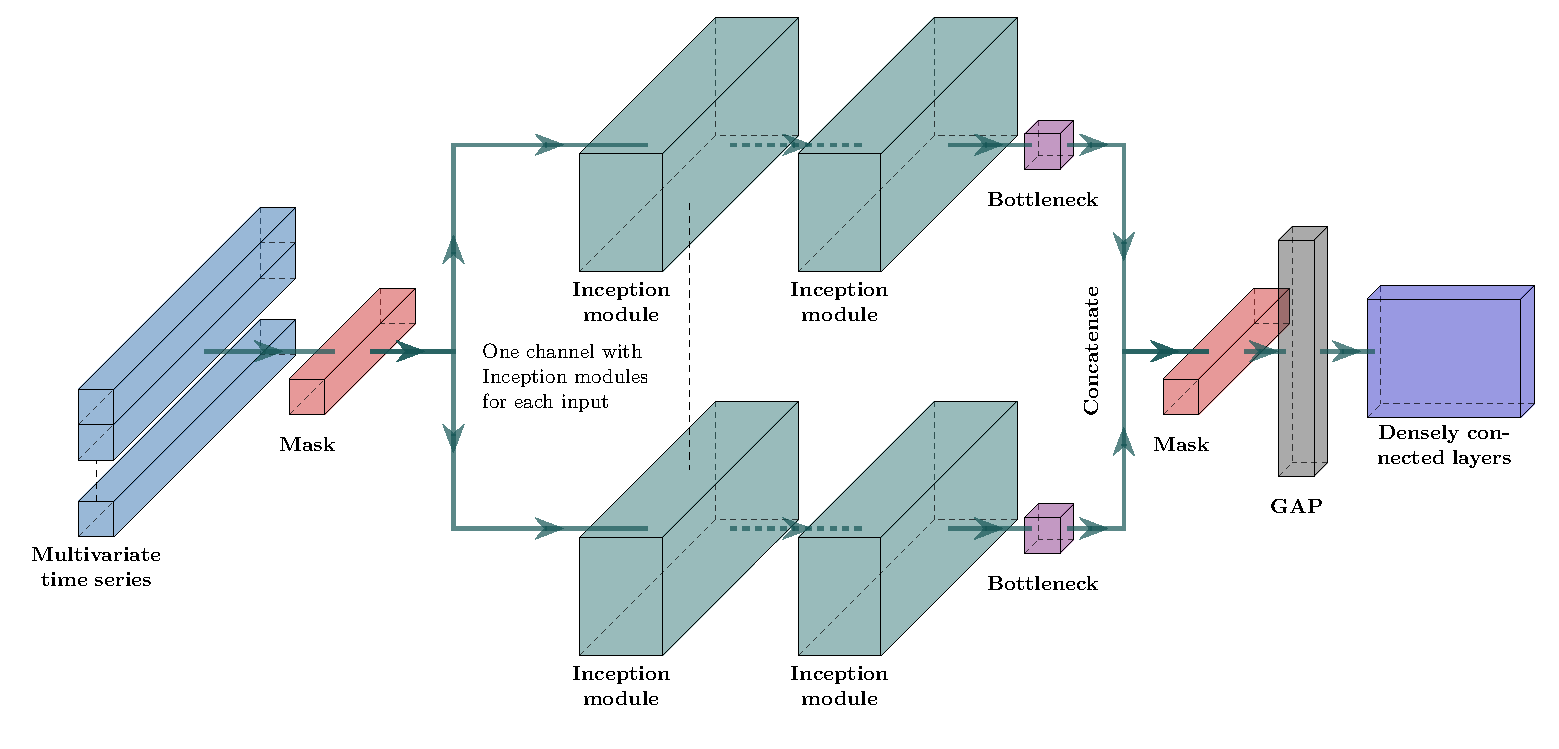
\includegraphics[width=\textwidth]{files/figs/x-inception.pdf}
  \caption{}
  \label{}
\end{figure}
